\subsection{Onda completa de puente}
El circuito con filtro de $470[\mu\text{F}]$ pueden verse en la
\textbf{figura~\ref{circuito07}} para el rectificador de onda completa de
puente.

\begin{figure}[!h]
\centering
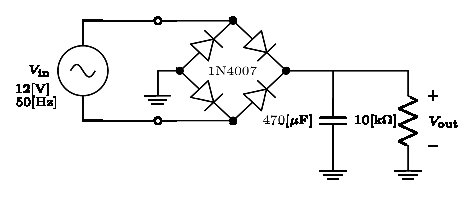
\includegraphics[scale=1.1]{diagramas/07.onda_completa2.eps}
\caption{Rectificador de onda completa con puente y filtro.}
\label{circuito07}
\end{figure}

\subsubsection{Simulación}
Se utilizó el software \emph{Quite Universal Circuit Simulator.} versión 23.3.1
para la simulación del rectificador de onda completa con filtro, este puede
verse en la \textbf{figura~\ref{simulacion07}}.

\begin{figure}[!h]
\centering
\includegraphics[scale=0.75]{simulacion/07.onda_completa2.eps}
\caption{Simulación del rectificador de onda completa con puente y filtro.}
\label{simulacion07}
\end{figure}

\subsubsection{Laboratorio}
Se presenta el rectificador de onda completa con puente y filtro armado en
laboratorio y su medición de voltaje de salida en la carga, en la
\textbf{figura~\ref{laboratorio09}}.

\begin{figure}[!h]
\centering
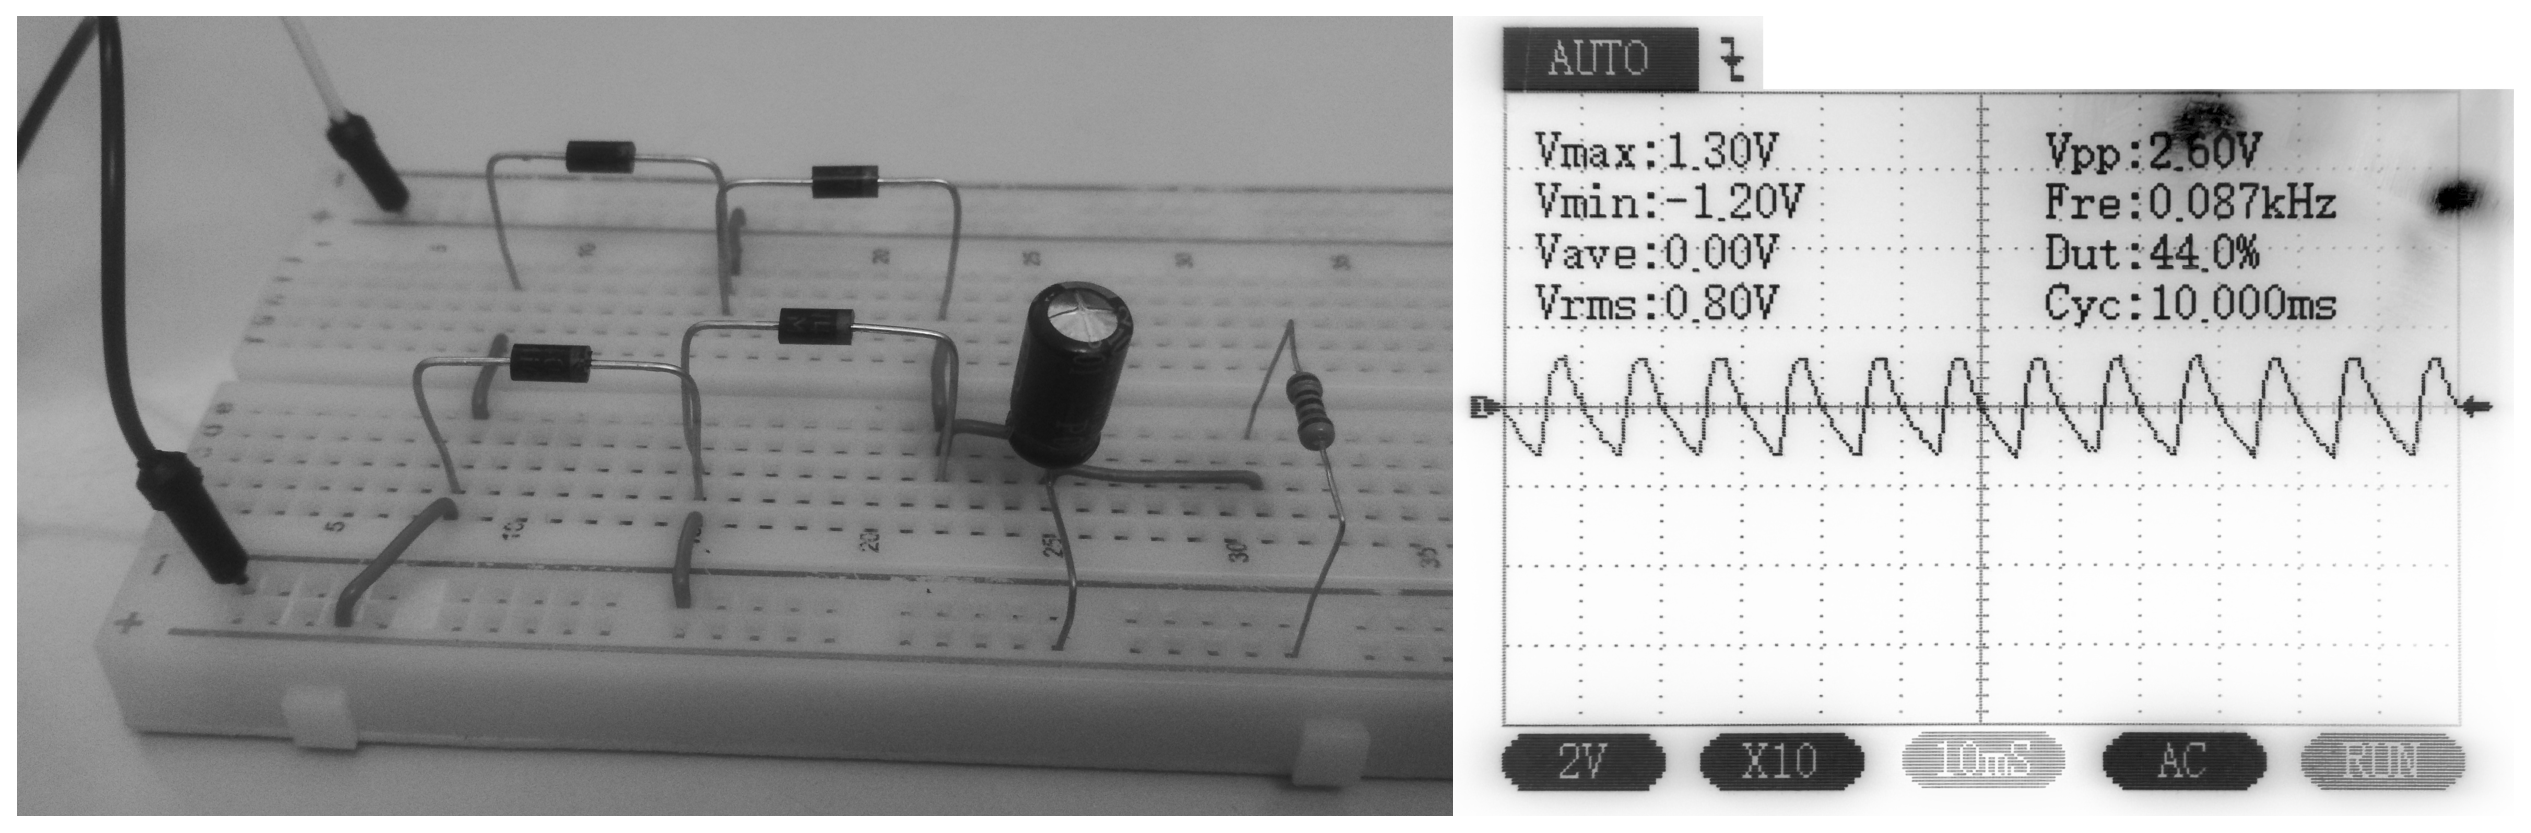
\includegraphics[scale=0.34]{fotos/07.onda_completa2.eps}
\caption{Rectificador de onda completa con puente y filtro.}
\label{laboratorio09}
\end{figure}

